\qrchapter{https://forgottenpillar.com/rsc/pl-fp-chapter12}{Rzeczywistość nieba}

\emcap{Osobowość Boga} dotyczy właściwości lub stanu Boga jako osoby. Ilekroć patrzymy na pracę pionierów dotyczącą \emcap{osobowości Boga}, widzimy, że wszyscy byli zgodni co do poglądu, że Bóg jest namacalną \textit{istotą}, posiadającą zarówno ciało, jak i części ciała. Zawsze widzimy to samo podstawowe rozumowanie, które odróżnia termin ‘\textit{duch}’ od terminu ‘\textit{istota}’. Rozróżniając te terminy, wyjaśniają właściwość lub stan Boga jako osoby\footnote{\href{https://www.merriam-webster.com/dictionary/personality}{Słownik Merriam-Webster} definiuje słowo ‘\textit{personality}’ jako “\textit{właściwość lub stan jako osoby}”.} — \emcap{osobowość Boga}. Wszystkie ich wnioski są podsumowane w pierwszym punkcie \emcap{Fundamentalnych Zasad}. \others{Jest \textbf{jeden Bóg}, \textbf{osobowa}, \textbf{duchowa istota}, Stwórca wszystkich rzeczy, wszechmogący, wszechwiedzący, … i \textbf{wszędzie obecny przez swojego przedstawiciela, Ducha Świętego}. Ps 139:7.}[FPSDA 1.2][https://egwwritings.org/read?panels=p1299.6]

Do tej pory w pracach pionierów widzieliśmy, że \emcap{osobowość Boga} jest ściśle związana z rzeczywistością Bożej obecności. Bóg jest osobową duchową istotą, mającą ciało i kształt; w związku z tym Jego obecność jest ograniczona do jednego miejsca — jak mówi Biblia, do Jego świątyni, przy Jego tronie, gdzie otacza Go niedostępna chwała. Jednak jest wszędzie obecny przez swojego przedstawiciela, Ducha Świętego. Oczywiście Duch Święty jest duchem, a nie istotą, \bible{bo duch nie ma ciała ani kości, jak widzicie, że ja mam}, powiedział Jezus (Łk 24:39). Chrystus jest również Istotą, jak Jego Ojciec. Jest dokładnym obrazem osoby Ojca; dlatego ma tę samą osobowość, czyli właściwość lub stan jako osoby, co Jego Ojciec.

W naszym doświadczeniu, gdy przedstawiamy pierwotne wierzenia Adwentystów Dnia Siódmego dotyczące \emcap{osobowości Boga} naszym trynitarnym braciom, wyrażone w pierwszych dwóch punktach \emcap{Fundamentalnych Zasad}, często twierdzą oni, że stwierdzenia w \emcap{Fundamentalnych Zasadach} są w pewien sposób poprawne, ale rozumienie przypisane terminom „\textit{osobowa duchowa istota}” jest błędne. Zwykle próbują zharmonizować \emcap{Fundamentalne Zasady} z doktryną o Trójcy poprzez przekręcanie słów „\textit{duchowa istota}”, jakby słowo ‘\textit{duchowa}’ oznaczało coś tajemniczego, odpowiedniego do zrównania \emcap{osobowości Boga} i Chrystusa z osobowością Ducha Świętego\footnote{Właściwość lub stan Ducha Świętego jako osoby polega na dawaniu świadectwa, a nie na posiadaniu postaci osoby. \egw{\textbf{Duch Święty ma osobowość}, \textbf{\underline{inaczej} nie mógłby \underline{świadczyć} naszemu duchowi} i z naszym duchem, że jesteśmy dziećmi Bożymi. \textbf{Musi On również być boską osobą}, \textbf{\underline{inaczej} nie mógłby \underline{badać} tajemnic, które są ukryte w umyśle Boga}. «Bo któż z ludzi wie, co jest w człowieku, oprócz ducha ludzkiego, który w nim jest? Tak samo i tego, co jest w Bogu, nikt nie wie, oprócz Ducha Bożego». [1Kor 2:11.]}[21LtMs, Ms 20, 1906, par. 32][https://egwwritings.org/read?panels=p14071.10296041&index=0]. Jest krystalicznie jasne, że Duch Święty jest osobą, jednak nie w ten sam sposób co Ojciec i Syn, ponieważ Duch Święty nie posiada właściwości zewnętrznej fizycznej osobowości jak Ojciec i Syn.}. Podstawowy problem sprowadza się do zrozumienia niebiańskich rzeczywistości. Biblia nie milczy w temacie nieba i jego rzeczywistości, a nasi pionierzy dobrze to rozumieli. Poniżej czytamy wyjaśnienie terminów „\textit{duchowa istota}” przez Jamesa White'a i Uriaha Smitha w ich książce \textit{The Biblical Institute}. Biblia wyjaśnia te terminy na przykładzie aniołów, którzy są „\textit{duchowymi istotami}”.

\begin{figure}[hp]
    \centering
    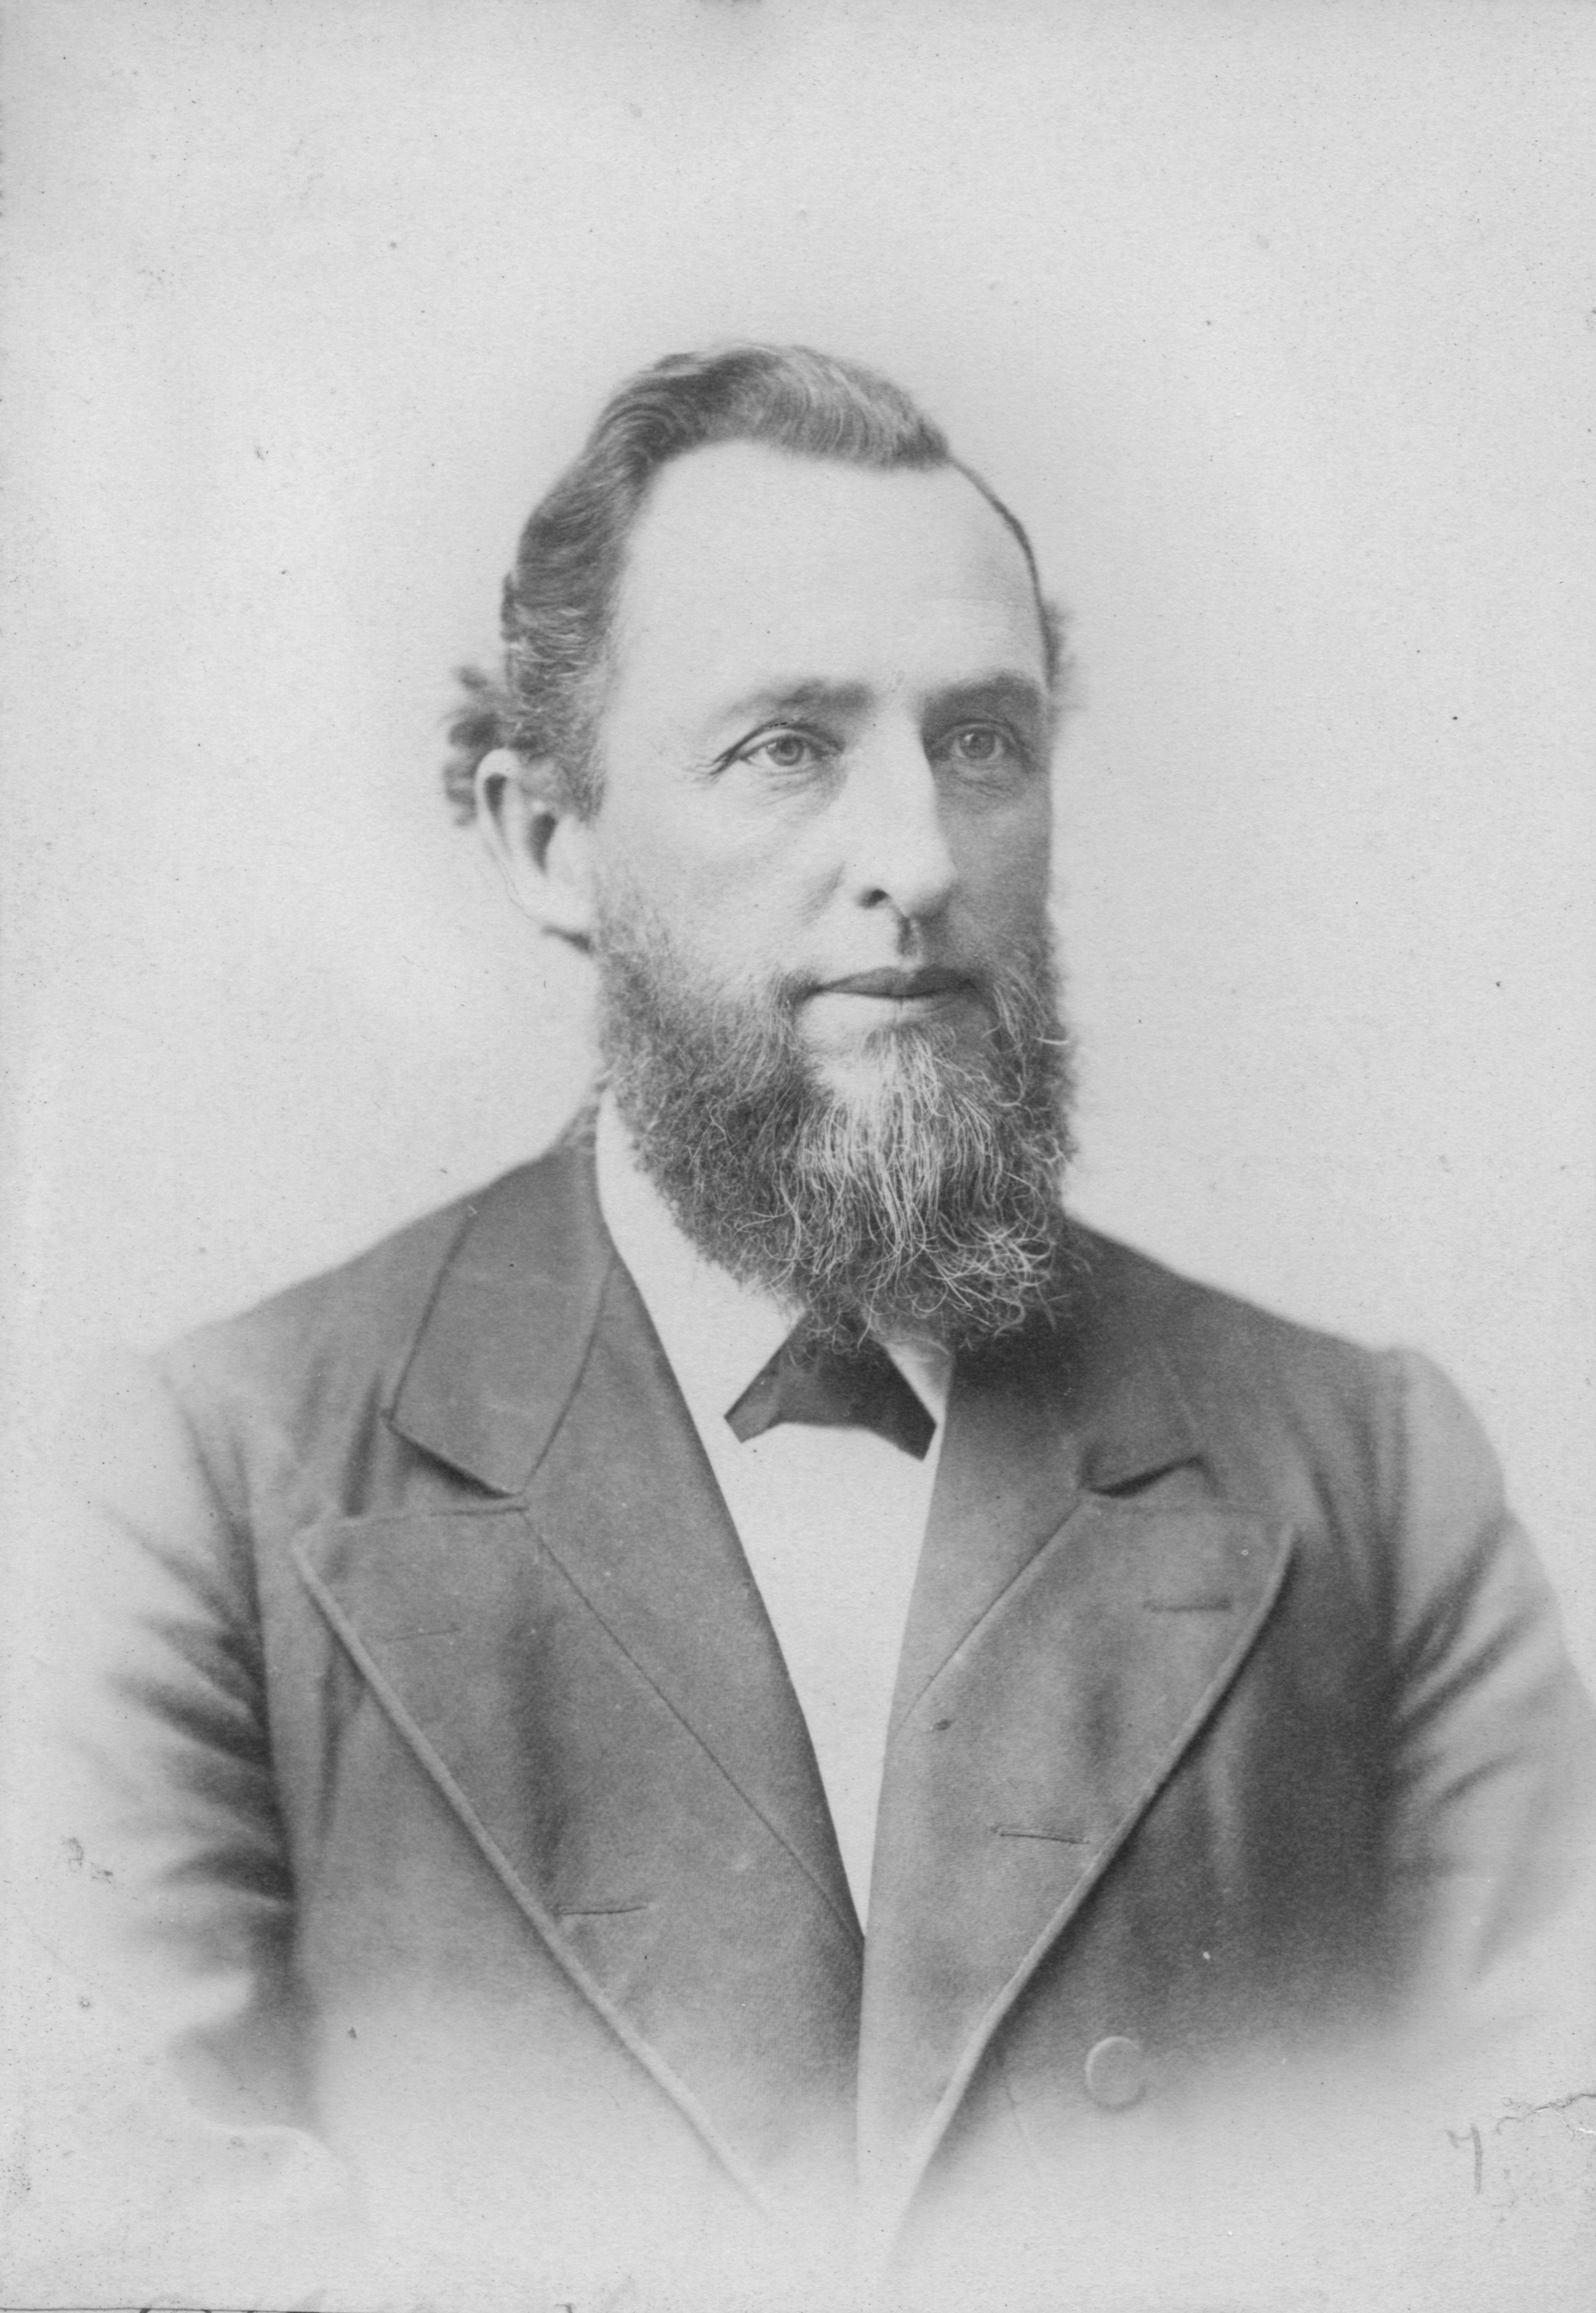
\includegraphics[width=1\linewidth]{images/uriah-smith.jpg}
    \caption*{Uriah Smith (1832-1903)}
    \label{fig:uriah-smith}
\end{figure}


\others{\textbf{Aniołowie są rzeczywistymi istotami}. Są opisani w Biblii jako \textbf{posiadający m.in. twarz, stopy, skrzydła}. Ezechiel mówi o cherubinach: «\textbf{Całe ich \underline{ciało}, ich plecy, ich ręce i ich skrzydła}... Ez 10:12. Aniołowie \textbf{ukazali się} Abrahamowi. Rdz 18:1--8. Rozmawiali i jedli z nim. Poszli do Sodomy i rozmawiali z Lotem, który wszedłszy do swego domu, upiekł dla nich przaśny chleb, a oni jedli. \textbf{Te osoby były nazywane aniołami}. Dawid mówi o mannie jako o zbożu z Nieba i pokarmie aniołów. Ps 78:23--25.}

\othersnogap{Przypadek Balaama, Lb 22:22--31, jest interesującym zdarzeniem. Anioł \textbf{ukazał się} Balaamowi z \textbf{wyciągniętym mieczem w ręku}. Czasami zadawane jest pytanie, \textbf{jak aniołowie mogą być \underline{materialnymi istotami, skoro nie możemy ich zobaczyć}. Ten przypadek to ilustruje}. Zapis mówi, że \textbf{Pan otworzył oczy Balaama i zobaczył on anioła}. \textbf{Anioł nie stworzył ciała na tę okazję}. \textbf{Był dokładnie taki sam jak przed tym, gdy Balaam go zobaczył; \underline{ale zmiana zaszła w Balaamie}}. Jego oczy zostały otwarte i wtedy ujrzał anioła. Tak samo było ze sługą Elizeusza, gdy on i jego pan znaleźli się w trudnym położeniu, otoczeni przez armię króla Syrii. 2Krl 6:17. Elizeusz modlił się, aby \textbf{oczy jego sługi zostały otwarte}; i natychmiast zobaczył on całą górę pełną koni i rydwanów wokół Elizeusza.}

\othersnogap{\textbf{Można to dalej zilustrować odnosząc się do rzeczy, o których wiemy, że są materialne, a jednak których nie możemy zobaczyć}. Powietrze jest materialne, światło jest materialne, nawet myśl sama w sobie jest tylko wynikiem materialnych reakcji — materią działająca na materię — a jednak nie możemy zobaczyć żadnej z tych rzeczy. \textbf{Tak samo jest z aniołami}.}

\othersnogap{\textbf{Dalszym zarzutem wobec materialności aniołów jest to, że są nazywani duchami}. Hbr 1:13--14. \textbf{\underline{Lecz to nie jest zarzut przeciwko temu, że są dosłownymi istotami}}. \textbf{Są po prostu duchowymi istotami skonstruowanymi inaczej niż te ziemskie ciała, które posiadamy}. Paweł mówi, 1Kor 15:44: «\textbf{Jest ciało cielesne i jest \underline{ciało duchowe}}». \textbf{Ciało cielesne mamy teraz; ciało duchowe będziemy mieli przy zmartwychwstaniu}. «\textbf{Jest wskrzeszane jako ciało duchowe}». Werset 44. \textbf{Wtedy będziemy równi aniołom}, Łk 20:36; \textbf{wtedy będziemy mieli ciała podobne do najchwalebniejszego ciała Chrystusa}, Flp 3:4, \textbf{a Chrystus nie jest mniej duchem niż aniołowie}. \textbf{Czytamy, że Bóg jest duchem, to znaczy po prostu \underline{duchową istotą}}.}[James White and Uriah Smith, The Biblical Institute (Kindle Locations 2537-2553). Kindle Edition.]

Biblia daje nam wgląd w to, że aniołowie są duchowymi istotami, które posiadają materialne ciała, ale są dla nas niewidzialni, chyba że Pan otworzy nasze oczy, abyśmy ich zobaczyli. Kiedy sprawiedliwi powstaną w swoich nowych uwielbionych ciałach, powstaną w ciele duchowym, niezniszczalnym. To ciało będzie namacalne i materialne, tak jak nowa ziemia będzie namacalna i materialna. A w naszych duchowych ciałach posiądziemy odnowioną ziemię, będziemy ją \bible{napełniać i czynić ją sobie poddaną; i panować nad rybami morskimi i nad ptactwem niebieskim, i nad wszelką żywą istotą, która porusza się po ziemi}[Rdz 1:28].

% Rzeczywistość nieba

\begin{titledpoem}
    \stanza{
        Bóg nie jest tajemnicą, lecz Istotą prawdziwą, \\
        Na tronie nieba siedzi z chwałą niewątpliwą. \\
        Choć w jednym miejscu przebywa jako Osoba, \\
        Przez Ducha jest obecny, gdzie tylko potrzeba.
    }

    \stanza{
        Duchowa Istota z ciałem i kształtem, \\
        Nie bezcielesny duch, lecz Byt z majestatem. \\
        Syn jest Jego obrazem, tę samą ma naturę, \\
        Obaj są namacalni, to prawda, nie złudzenie.
    }

    \stanza{
        Aniołowie, jak Bóg, są istotami realnymi, \\
        Choć dla oczu śmiertelnych pozostają niewidzialnymi. \\
        Mają ciała duchowe, lecz materialne zarazem, \\
        Takie, jakie my otrzymamy zmartwychwstania obrazem.
    }
\end{titledpoem}

\begin{titledpoem}
    \stanza{
        Niebiańska rzeczywistość nie jest mgłą tajemną, \\
        Lecz światem namacalnym z chwałą niepojemną. \\
        Bóg jako Osoba ma ciało i części, \\
        W jednym miejscu przebywa, lecz Duchem się mieści.
    }

    \stanza{
        Pionierzy adwentyzmu prawdę tę głosili, \\
        Że Bóg i Syn są Istotami, nie duchem bez siły. \\
        Duch Święty to przedstawiciel, nie trzecia Istota, \\
        To przez Niego Bóg działa, gdy pomoc jest potrzebna.
    }

    \stanza{
        Gdy zmartwychwstaniemy w ciałach duchowych, \\
        Będziemy jak aniołowie w kształtach gotowych. \\
        Materialni, namacalni, choć duchowej natury, \\
        Zamieszkamy na ziemi nowej, bez śmierci ponurej.
    }
\end{titledpoem}

\begin{titledpoem}
    \stanza{
        Bóg jest Istotą, nie abstrakcyjną mocą, \\
        Ma kształt i formę, nie jest bezcielesną nocą. \\
        Osobowość Jego to stan bycia Osobą, \\
        Ograniczoną miejscem, lecz z Ducha swobodą.
    }

    \stanza{
        Oczy Balaama ujrzały anioła dopiero, \\
        Gdy Pan je otworzył na prawdę i szczerość. \\
        Tak samo my ujrzymy niebiańskie istoty, \\
        Gdy Bóg nam pozwoli przeniknąć zasłony.
    }

    \stanza{
        Ciało duchowe to nie duch bez ciała, \\
        Lecz byt materialny, którego moc trwała. \\
        W takich ciałach będziemy na nowej ziemi żyli, \\
        Namacalnej, realnej, gdzie Boga będziemy czcili.
    }
\end{titledpoem}
